
Nelle applicazioni è di uso frequente una formula empirica per calcolare le perdite
chiamata formula di Steinmetz (1892)
$$
P_{\text{ist}} = K_\text{ist}\cdot B^\alpha_\text{max}\ f
$$
dove $\alpha$ è tipicamente $1.6$ mentre il coefficiente di isteresi $K_\text{ist}$ dipende
dalla grandezza specifica che si vuole indicare se $\si{\watt\per\meter^3}$ o $\si{\watt\per\kilo\gram}$. La seconda è tipicamente utilizzata in ingegneria elettrica
e denominata \textit{cifra di perdita}, dipende esclusivamente dal materiale.

Il materiale utilizzato nelle macchine elettriche, solitamente Fe-Si possiede 
un'area del ciclo di isteresi inferiore a quella del ferro puro a parità di $M_s$ 
magnetizzazione di saturazione.

\subsection{Misura del ciclo di isteresi di un materiale}
Si utilizzerà un mezzo sperimentale composto da vari blocchi, partendo dall'alimentazione
di rete si utilizza un VARIAC, un autotrasformatore abbassatore in questo caso
che fornisce al sistema una tensione minore o uguale a quella di alimentazione.

Si effettuano infine due avvolgimenti destrorsi al campione ferromagnetico da studiare
$N_1$ ed $N_2$ in base al numero di spire. Ai terminali di $N_2$ si collega un ``blocco
integratore'' costituito da un resistore in serie e un capacitore in derivazione.

Utilizzando un oscilloscopio è poi possibile visualizzare la corrente al ``primario''
proporzionale alla tensione sul resistore di misura e quella al secondario misurata
ai capi del condensatore.
\begin{figure}[H]
\centering
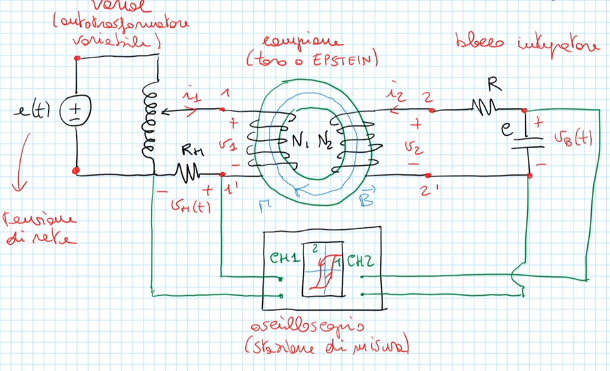
\includegraphics[width = 0.7\linewidth]{misurazione_isteresi_toro}
\end{figure}

Per studiare il funzionamento del circuito si applica la legge di Ampere ad una generica 
linea $\Gamma$ interna al toroide
$$
\oint_\Gamma \vec{H}\cdot\hat{t} dl = N_1 i_1 + N_2 i_2 = 2\pi r H
$$
supponendo che $\vec{H}$ e $\vec{B}$ siano entrambi confinati nel toro e quindi paralleli

Si assume di dimensionare la resistenza R in modo tale che $N_2 i_2 \ll N_1i_1 $, in questo 
modo
$$
N_1 i_1 \simeq 2\pi r H \Rightarrow H \simeq \frac{N_1 i_1}{2 \pi r}
$$

Si suppone inoltre che il raggio maggiore del toro $a\gg \sqrt{S}$ dove $S$ è l'area della
sezione trasversa del toro, allora il raggio generico interno al toro è approssimabile 
al suo raggio massimo $r\simeq a \Rightarrow H\simeq \frac{N_1i_1}{2\pi a}$.

Per ricavare invece il campo $\vec{B}$ si utilizza la legge di Faraday-Neumann, immaginando
di ingrandire la regione del toro sulla quale è avvolta la spira $N_2$ e si suppone una 
linea $\Gamma_2$ che percorre l'avvolgimento, assumendo che il conduttore sia perfetto.
\begin{figure}[H]
\centering
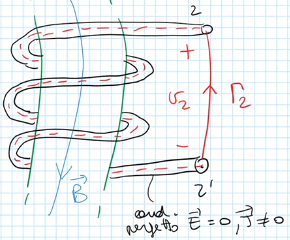
\includegraphics[width = 0.5\linewidth]{misurazione_b_isteresi_toro}
\end{figure}
$$
\oint_{\Gamma_2} \vec{E}\cdot\hat{t}dl = -\frac{d}{dt} \Phi_{\Gamma_2} = -\frac{d}{dt} \iint_{S_{\Gamma_2}}\vec{B}\cdot\hat{n}dS
$$
il contributo è valutabile solo nella regione aperta della linea $\Gamma_2$
$$
\int_{2'\Gamma_2 2} \vec{E}\cdot\hat{t}dl = -v_2 = - \frac{d\Phi_2}{dt}\Rightarrow v_2 = \frac{d\Phi_2}{dt} = N_2 S \frac{dB}{dt}
$$
Se si suppone che il campo $\vec{B}$ sia interamente confinato nel toro, non interessa
la forma della curva $\Gamma_2$ all'esterno dell'avvolgimento che lo circonda.

Se $v_2$ è proporzionale alla derivata del campo $\vec{B}$ è necessario dunque
integrarla per ottenere il campo, si utilizza un circuito RC integratore.
\begin{figure}[H]
\centering
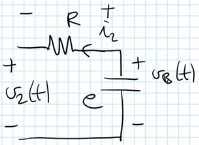
\includegraphics[width = 0.3\linewidth]{integratore_RC_campo_H}
\end{figure}
$$
\begin{aligned}
& v_2(t) +Ri_2 = v_B(t)\\
& v_2(t) - RC\frac{dv_B}{dt} = v_B(t)
\end{aligned}
\Rightarrow v_2(t) = \tau \frac{dv_B}{dt} + v_B(t)
$$
$$
v_B(t) = v_{B\text{ lib}}(t) + v_{B\text{ forz}}(t) = v_B(0)e^{-\frac{t}{\tau}} + \int_0^t 
v_2(t')h(t-t')dt'
$$
$$
h(t) = -\frac{1}{RC} e^{-\frac{t}{RC}} = -\frac{1}{\tau} e^{-\frac{t}{\tau}}
$$
$$
v_B(t) = v_B(0) e^{-\frac{t}{\tau}} - \frac{1}{\tau} \int_0^t v_2(t') e^{-\frac{(t-t')}{\tau}} dt' =  v_B(0) e^{-\frac{t}{\tau}} - \frac{1}{\tau}e^{-\frac{t}{\tau}} \int_0^t v_2(t') e^{\frac{t'}{\tau}} dt'
$$

Se il tempo di integrazione $t \ll \tau \Rightarrow e^{-\frac{t}{\tau}}=1$ si può approssimare l'equazione
$$
v_B(t) \simeq v_B(0) - \frac{1}{RC} \int_0^t v_2(t') dt'
$$
Se invece $v_B(t)$ fosse sinusoidale e $\omega\tau \gg 1$ si avrebbe
$$
\overline{V}_2 = j\omega\tau \overline{V}_B + \overline{V}_B \simeq j\omega \tau \overline{V}_B
$$
ossia nel dominio dei fasori sarebbe immediato dimostrare che $\overline{V}_B$ sia 
l'integrale di $\overline{V}_2$

Se $v_B(0) = \SI{0}{\volt}$ 
$$
v_B(t) = -\frac{1}{RC} \int_0^t v_2(t') dt' = -\frac{1}{RC}\Phi_2 = -\frac{1}{RC} N_2\ S\ B 
$$

In conclusione si riportano le due tensioni misurate dall'oscilloscopio
\begin{align*}
v_B(t) &= -\frac{1}{RC}N_2 S \cdot B(t) \\
v_H(t) &= R_H \frac{2\pi a }{N_1} \cdot H(t)
\end{align*}

Riportando $v_H$ sull'asse delle ascisse e $v_B$ su quello delle ordinate è possibile
visualizzare il ciclo di isteresi.

\newpage
\subsection{Circuiti magnetici}
È possibile studiare i circuiti magnetici mediante un'analogia con i circuiti elettrici,
si riprende per questo motivo il modello della conduzione stazionaria.
$$
\begin{cases}
\oiint_\Sigma \vec{J}\cdot\hat{n} dS = 0\qquad \forall\ \Sigma\\
\oint_\Gamma \vec{E}\cdot \hat{t} dl = 0\qquad\quad \forall\ \Gamma \\
\vec{J} = \gamma\left(\vec{E}+\vec{E}_m\right)
\end{cases}
\Leftrightarrow
\begin{cases}
\oiint_\Sigma \vec{J}\cdot\hat{n} dS = 0 \\
\oint_\Gamma \left(\vec{E}+\vec{E}_m\right)\cdot\hat{t}\ dl = \oint_\Gamma \vec{E}_m\cdot\hat{t}\ dl = \mathcal{E}_\Gamma\\
\vec{J} = \gamma\vec{E}_T
\end{cases}
$$
avendo definito $\vec{E}_T = \vec{E} + \vec{E}_m$ e ricordando che $\mathcal{E}_\Gamma$ è
la forza elettromotrice sulla linea $\Gamma$.

Si compara il modello della conduzione stazionaria con quello della magnetostatica
e si vedono delle evidenti corrispondenze tra i termini, anche se essi sono entità fisiche 
differenti
$$
\left\{\begin{aligned}
&\oiint_\Sigma \vec{J}\cdot\hat{n}dS = 0\\
& \oint_\Gamma \vec{E}_t\cdot\hat{t}dl = \mathcal{E}_\Gamma \\
&\vec{J} = \gamma \vec{E}_T
\end{aligned}
\right.
\quad
\left\{\begin{aligned}
&\oiint_\Sigma \vec{B}\cdot\hat{n}dS = 0\\
& \oint_\Gamma \vec{H}_t\cdot\hat{t}dl = i_\Gamma \\
&\vec{B} = \mu \vec{H}
\end{aligned}
\right.
\quad
\left\{\begin{aligned}
&\vec{B} \leftrightarrow \vec{J}\\
&\vec{H} \leftrightarrow \vec{E}_T \\
& i_\Gamma \leftrightarrow \mathcal{E}_\Gamma
\end{aligned}
\right.
$$
È necessario però evidenziare anche le differenze tra i due modelli
Un circuito elettrico è un tubo di flusso per $\vec{J}$, 
$\hat{n}\cdot(\vec{J}_2-\vec{J}_1) = 0$, questa cosa non è vera per $\vec{B}$ in quanto
presente in tutto lo spazio, anche se si considera un'interfaccia con due differenti $\mu$,
la componente tangente di $\vec{H}$ è sempre continua e quindi $\frac{B_{t_2}}{\mu_2} = \frac{B_{t_1}}{\mu_1}$ mentre la componente normale di $\vec{B}$ è continua e quindi $B_{n_1} = B_{n_2}$.
\begin{figure}[H]
\centering
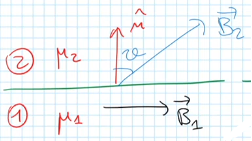
\includegraphics[width = 0.5\linewidth]{continuita_campo_normale_B}
\end{figure}
Con queste considerazioni si può affermare
$$
\frac{B_{t_2}}{B_{n_2}}\frac{1}{\mu_2} = \frac{B_{t_1}}{B_{n_1}}\frac{1}{\mu_1} \Rightarrow 
\frac{\tan \theta_2}{\mu_2} = \frac{\tan\theta_1}{\mu_1}\Rightarrow \tan\theta_2 = \frac{\mu_2}{\mu_1}\tan\theta_1
$$
Quella ottenuta è la legge della rifrazione magnetica e si vede che il campo $\vec{B}$ può
essere tangente ad $S$ solo se il rapporto $\frac{\mu_2}{\mu_1}\to 0$ ma questo non è 
praticamente possibile dato che il minimo valore di permeabilità è quello del vuoto
e il valore più alto si ha invece nei materiali ferromagnetici che hanno una permeabilità
pari a circa \SI{e3} o \SI{e4} volte $\mu_0$.
\newpage

Il ferro dolce presenta un ciclo di isteresi stretto, approssimabile alla sua
linea media se il materiale lavora nella zona di non saturazione. Si definisce una 
permeabilità differenziale $\frac{dB}{dH} = \mu_r\mu_0$ e approssimare il materiale
ferromagnetico ad un mezzo lineare.
1:29:22
